\documentclass[UTF8]{ctexart}
\usepackage{subfigure}
\usepackage{caption}
\usepackage{amsmath,bm}
\usepackage{amssymb}
\usepackage{pifont}
\usepackage{geometry}
\usepackage{graphicx}
\usepackage{gensymb}
\usepackage{wrapfig}
\usepackage{titlesec}
\usepackage{float}
\usepackage{diagbox}
\usepackage{fancyhdr}
\usepackage{color}
\usepackage{bm}
\usepackage{siunitx}
\usepackage{ulem}
\usepackage{CJKulem}
\pagestyle{plain}
\geometry{a4paper,scale=0.8}
\CTEXsetup[format+={\raggedright}]{section} 
\title{操作系统2017期末}
\author{Deschain}
\titlespacing*{\section}
{0pt}{0pt}{0pt}
\titlespacing*{\subsection}
{0pt}{0pt}{0pt}
\titlespacing*{\paragraph}
{0pt}{0pt}{0pt}
\titlespacing*{\subparagraph}
{0pt}{0pt}{0pt}
\titleformat*{\section}{\normalsize}
\titleformat*{\subsection}{\normalsize}
\begin{document}
\maketitle
\section*{一、简答题(每题5分,共计40分)}
\subsection*{1.程序和进程有何区别?}
进程时程序的一次运行活动,包含数据、资源等。程序只是一段代码。\\
\subsection*{2.在操作系统中为什么要引入线程?如何实现线程?}
(1)引入:使多个程序能够并发执行,提高资源利用率和系统吞吐量。\\
(2)实现:用户级线程、内核级线程、混合实现。\\
\subsection*{3.实时系统中的RM和EDF调度算法的基本思想是什么?}
(1)RM:先执行优先级最高的就绪进程,必要时抢先当前进程。\\
(2)EDF:优先执行截止时限最早的进程。\\
\subsection*{4.在I/O设备的控制方式中,中断方式和DMA方式的区别是什么?}
DMA大大减少了CPU进行中断处理的次数。
\subsection*{5.在内存管理中,什么是内碎片?什么是外碎片?请举例说明?}
(1)内碎片:占用分区之内未被利用的空间。\\
(2)外碎片:占用分区之间难以利用的空闲分区。\\
\begin{figure}[H]                                         
    \centering                                                
    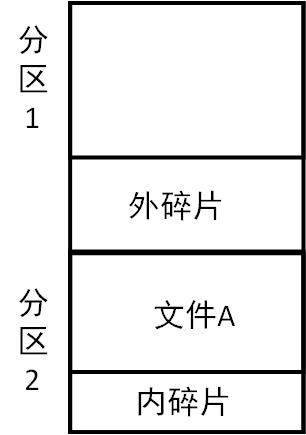
\includegraphics[width=4cm,height=6cm]{ans-1-5.jpg}        
    \caption*{}                                                                                   
\end{figure}
\subsection*{6.在文件的物理结构中,链接结构和索引结构各有什么优缺点?}
(1)链接结构\ding{172}优点:充分利用磁盘空间;没有外碎片;顺序访问速度快;\ding{173}缺点:随机访问性能差;较多的寻道次数和
寻道时间;由于指针占去一些字节,数据部分不再是2的整数幂次。\\
(2)索引结构\ding{172}优点:既能随机存取,又能顺序存取;满足了文件动态增长、插入删除的需求;能充分利用外存空间;\ding{173}
较多的寻道次数和寻道时间;索引表本身带来了系统开销。\\
\subsection*{7.在I/O设备管理中,为什么要引入缓冲技术?}
CPU速度比外设快得多,两者的并行程度不能得到充分发挥。\\
\subsection*{8.什么是死锁?死锁的必要条件有哪些?}
(1)系统内多个进程无限制地等待永远不会发生的条件。\\
(2)互斥、非抢占、请求和保持、环路等待。\\
\section*{二、综合应用题(每题15分,共计60分)}
\subsection*{1.在具有单一CPU和两台输入/输出设备DEV1,DEV2的多道程序设计环境下,有3个作业Job1、Job2、Job3同时投入运行。这三
个作业对CPU和输入/输出设备的使用顺序和时间如下:\\
Job1:DEV2(30ms)、CPU(10ms)、DEV1(30ms)、CPU(10ms)、DEV2(20ms)\\
Job2:DEV1(20ms)、CPU(20ms)、DEV2(40ms)\\
Job3:CPU(30ms)、DEV1(20ms)、CPU(10ms)、DEV1(10ms)\\
假设CPU、DEV1、DEV2都能并行工作,作业的优先级高低为Job1>Job2>Job3,优先级高的作业可以抢占优先级低的作业的CPU,但是不可抢占输
入/输出设备。试求:\\
(a)三个作业的平均周转时间;\\
(b)CPU的利用率;\\
(c)DEV1和DEV2的利用率;\\
}
(a)$\frac{1}{3}(70+90+110)=90ms$\\
(b)$\frac{7}{11}$\\
(c)DEV1:$\frac{8}{11}$DEV2:$\frac{7}{11}$\\
\subsection*{2.在某单CPU的系统中,某一时刻就绪队列中按序排列有5个进程A、B、C、D和E,其所需运行时间和优先级如下表所示,其中优先级数字越小表示优先级越高。\\
\begin{tabular}{|c|c|c|}                      
    \hline                                        
   进程&所需运行时间&优先级\\
    \hline
    A&3&3\\
    \hline                                      
    B&7&5\\                                    
    \hline
    C&5&1\\
    \hline
    D&2&4\\
    \hline
    E&6&2\\
    \hline
\end{tabular}
对下述调度算法计算平均周转时间:\\
(a)最高优先级优先;\\
(b)先来先服务;\\
(c)短作业优先;\\
(d)时间片轮转(时间片为1);\\
(e)时间片轮转(时间片为2)。\\
}
(a)$\frac{1}{5}(14+23+5+16+11)=13.8$\\
(b)$\frac{1}{5}(3+10+15+17+23)=13.6$\\
(c)$\frac{1}{5}(2+5+10+16+23)=11.2$\\
(d)$\frac{1}{5}(11+23+19+9+22)=16.8$\\
(e)$\frac{1}{5}(11+23+20+8+22)=16.8$\\
\subsection*{3.某进程在运行时按顺序访问如下界面:2,3,1,6,5,,,,7,8,9,3,6,2,1,3,4,4,3,4,4,4。所有内存页最初都是空的,所以,凡第一次访问的页面都产生
一次缺页。\\
(a)进程分配有4个页框,采用FIFO算法,求缺页次数;\\
(b)进程分配有4个页框,采用LRU算法,求缺页次数;\\
(c)进程分配有4个页框,采用Clock算法,求缺页次数;\\
(d)设t为第12次页面访问的时刻,k=6,求工作集W(k,t);\\
(e)设t为第18次页面访问的时刻,k=6,求工作集W(k,t);\\
}
(a)13次\\
(b)12次\\
(c)12次\\
(d)W(k,t)=6\\
(e)W(k,t)=3\\
\subsection*{4.某小型餐厅为节约资源只提供了一间可以容纳2个人的卫生间,在使用卫生间时必须保证不能有不同性别的顾客同时出现在卫生间里。\\请利用信号量和P、
V操作编写一个程序来模拟卫生间的使用,你只需要写出伪代码,但是需要明确说明信号量的含义和初值。}








\end{document}